\documentclass[9pt]{beamer}
\usepackage[utf8]{inputenc}
\usepackage[english,russian]{babel}
\usepackage[UKenglish]{isodate}
\usepackage{amssymb,amsfonts,amsmath,cite,enumerate,float,indentfirst}
\usepackage{indentfirst}
\usepackage{cite}
\usepackage{amssymb}
\usepackage{wrapfig}
\usepackage{float}
\usepackage{amsthm}
\usepackage{graphicx}
\usepackage{grffile}
\usepackage{floatflt}
\usepackage[labelsep=period]{caption}
\usepackage{amsthm}
\usepackage{caption}
\usepackage{fancyhdr}
\usepackage{sidecap}
\usepackage{subcaption}
\usepackage{epstopdf} %for MikTex
\graphicspath{ {img/}}

\cleanlookdateon

\usetheme{Antibes}
\usecolortheme{seahorse}

\begin{document}
    \title{Reverse proplem of complex heat transfer}
    \author{Mesenev Pavel}\institute{Far Eastern Federal University}

    \date{2017}
\begin{frame}
    \titlepage
    \begin{minipage}{1\textwidth} % начало маленькой врезки в половину ширины текста
    \begin{flushleft} % выровнять её содержимое по левому краю
    \emph{scientific adv.:} Professor, Doctor of physical and mathematical sciences Chebotarev A. Yu.\\
    \emph{English language consultant:} Professor, Ph.D (philology), Gorodetskaya Ye. Ya.
    \emph{Department of} Informatics, mathematical and computer modelling\\
    \end{flushleft} % конец выравнивания по левому краю
    \end{minipage} % конец врезки
\end{frame}

\begin{frame}
\frametitle{mathematical model}

$\Omega \subset \mathbb{R}^2$ bounded domain with the boundary $\Gamma = \Gamma_0 \cup \Gamma_1 \cup \Gamma_2$.

Normalized steady-state model of heat transfer in  $\Omega$, has the following form:
\begin{equation}
    \label{initial}
    \begin{aligned}
                - a \Delta \theta + b \kappa_a(\theta ^ 3 | \theta | - \varphi) = 0,  \\
                - \alpha \Delta \varphi + \kappa_a (\varphi - \theta ^3 | \theta |) = 0,
    \end{aligned}
    \qquad \text{in } \Omega.
\end{equation}

\begin{equation}
    \label{initial_boundary}
    \begin{aligned}
        \Gamma: \; a \partial_n \theta + \beta (\theta - \theta _b) = 0, \\
        \Gamma_0 \ \cup \Gamma_2: \; \alpha \partial_n \varphi + \gamma(\varphi - \theta_b ^4 ) = 0, \\
        \Gamma_1: \; \alpha \partial_n \varphi + u(\varphi - \theta_b ^4 ) = 0, \\
    \end{aligned}
\end{equation}
$\theta$ is the normalized temperature, $\varphi$ the normalized radiation intensity averaged over all directions,  $\kappa_a$ the absorption coefficient. Constants $a, b, \alpha, \gamma, \beta$ и $\theta_b$ are given.

    Quality functional:
    \begin{equation}
    	\label{quality}
    	\mathcal{J}(\theta) = \frac{1}{2} \int_\Gamma (\theta - \theta_0)^2_d\Gamma \rightarrow inf
    \end{equation}
    Here $ \theta_0  \in L^2(\Gamma)$ defined functions.
\end{frame}

\begin{frame}
    Denote $H = L^2(\Omega), V = H^1(\Omega), Y = V \times V $.
    Define operators $A_{1,2}, \; F, f$
    $$A_{1,2}\colon V \to V', \; F \colon V \times U \to V',$$
    $$(A_1,\theta,v) = a( \nabla \theta, \nabla v ) + \int_\Gamma \gamma \theta v d\Gamma, (A_2 \varphi, v) = \alpha (\nabla \varphi,\nabla v),$$
    $$(F(\varphi, u), v) = \int_\Gamma u (\varphi - \theta ^4_b)v d\Gamma, \;  (f, v) = \int_\Gamma \gamma \theta_b v \Gamma$$

    A pair $\{\theta, \varphi \}$ is called weak solution of the problem (\ref{initial})--(\ref{quality}) if
    \begin{equation}
        \label{weak_operational}
        A_1 \theta + b \kappa_a (| \theta | \theta^3 - \varphi ) = f, A_2 \varphi + \kappa_a (\varphi - |\theta|\theta^3) + F(\varphi, u) = 0.
    \end{equation}

    The optimal control problem consists in the determination of the control $u$ and the corresponding state model:
        \begin{equation}
            \label{minimization_operational}
            J(\theta) \to \text{inf}, \; \{\theta, \varphi\} \text{ solution of \eqref{weak_operational}, with  } u \in U_{ad}
        \end{equation}
 \end{frame}

\begin{frame}
    (i) $ \beta,\gamma, u_1, u_2 \in L^\infty(\Gamma); \beta \ge \beta_0 > 0, \gamma \ge \gamma_0 > 0, 0 \le u_1 \le u_2;$

    (ii) $J(\theta) : V \times U_{ad} \rightarrow \mathbb{R}$ is weakly lower semicontinuous.

    (iii) $J(\theta) : V \times U_{ad} \rightarrow \mathbb{R}$ are Fréchet differentiable.

\begin{theorem}[Existence of optimal controls]
    Let $\hat{y}=\{\hat{\theta},\hat{\varphi} \} \in Y, \hat{u} \in U_{ad}$ is the solution of optimal controls problem. Then, there exists a pair $(\lambda, p) \in \mathbb{R}_{+} \times Y) \{0\}$
    such that $(\hat{y}, \hat{u}, p)$, where $p = (p_1, p_2)$ satisfies unequalities:
    \begin{equation}
    \label{therorem_2_eq1}
     A_1 p_1 + 4 \hat{\theta}^3 \kappa_a(b p_1 - p_2) = - \lambda J'_ \theta(\hat{y}),
    \end{equation}
    \begin{equation}
    \label{therorem_2_eq2}
        A_2 p_2 + \kappa_a (p_2-b p_1) + F_1( p_2, \hat{u}) = 0,
    \end{equation}
    \begin{equation}
    \label{therorem_2_eq3}
    \varepsilon \int_\Gamma u v + \int_\Gamma v p_2(\hat{\varphi} - \theta_b^4) \ge 0, \; v:= w - u, \; \forall w \in U_{ad}.
\end{equation}
$$ (F_1(p_2,\hat{u}),\zeta) = \int_\Gamma \hat{u} p_2 \zeta d \Gamma,\; \forall \zeta \in V.$$
\end{theorem}
\end{frame}

\section{Numerical experiments}
\begin{frame}
    \frametitle{Solution of the optimal control problem}
    \begin{itemize}
        \item Define an initial approximation for control function $u = u_0$
        \item Solve the primal problem \eqref{initial}--\eqref{initial_boundary}
        \item Solve the conjugate problems \eqref{therorem_2_eq1}--\eqref{therorem_2_eq2}
        \item By gradient descent method recalcuate control function $u$:
        $$u_{k+1} = P_{ad}\left[ u_k - \lambda (\varphi_k - \theta_b^4)p_{2k} \right].$$
    \end{itemize}
\end{frame}

\begin{frame}
\frametitle{Solution of the primal problem}
Find the solution $\{\theta, \varphi\}$ of \eqref{initial}--\eqref{initial_boundary} with the specified parameters.

The domain $\Omega = \{(x,y):x^2+y^2 \le 1\}$.
\begin{figure}[H]
    \centering
    \includegraphics[width=0.7\textwidth]{mesh_1.eps}
    \caption{Triangulation of $\Omega$}
\end{figure}

\end{frame}
\begin{frame}
\frametitle{Algorithm for solving the problem}
    \begin{itemize}
        \item Define the initial approximation for the pair $\{\theta, \varphi\}$
        \item Сalculation of the nonlinear term $\theta^3$
        \item Resolve by the finite element method the problem \eqref{weak_operational}
        \item The pair $\{\theta, \varphi\}$  obtained in the previous step is used as an approximation for the next iteration
    \end{itemize}
    \begin{figure}[H]
        \centering
        \includegraphics[width=0.5\textwidth]{iteration_dynamics.png}
        \caption{value $\|\theta_n - \theta_{n-1}\|_\Omega^2 + \|\varphi_n - \varphi_{n-1}\|_\Omega^2$}
    \end{figure}

\end{frame}

\begin{frame}
\frametitle{The results of the algorithm}
    For the experiment, the following system parameters were chosen:
    $ a = 0.3, \alpha = 0.6, \beta = 0,5,\gamma = 0.5, b = 0.5, \kappa_a = 0.8, \theta_b = x^2, u=0.5$
    \begin{figure}
        \begin{subfigure}[b]{0.5\textwidth}
        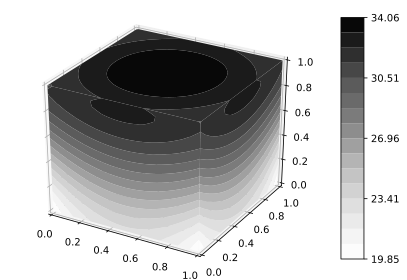
\includegraphics[width=\textwidth]{phi_final.eps}
        \caption{Function $\varphi$}
        \end{subfigure}%
        ~ %add desired spacing between images, e. g. ~, \quad, \qquad, \hfill etc.
          %(or a blank line to force the subfigure onto a new line)
        \begin{subfigure}[b]{0.5\textwidth}
        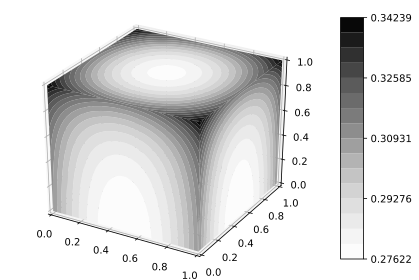
\includegraphics[width=\textwidth]{theta_final.eps}
        \caption{Function $\theta$}

        \end{subfigure}
        \caption{Solution of the primal problem \eqref{weak_operational}}
    \end{figure}
\end{frame}

\begin{frame}
\frametitle{The solution of the conjugate problem}

\begin{figure}
    \begin{subfigure}[b]{0.5\textwidth}
    \includegraphics[width=\textwidth]{pone.eps}
    \caption{Function $p_1$}
    \end{subfigure}%
    ~ %add desired spacing between images, e. g. ~, \quad, \qquad, \hfill etc.
      %(or a blank line to force the subfigure onto a new line)
    \begin{subfigure}[b]{0.5\textwidth}
    \includegraphics[width=\textwidth]{ptwo.eps}
    \caption{Function $p_2$}

    \end{subfigure}
    \caption{Solution of the conjugate problem \eqref{therorem_2_eq1}--\eqref{therorem_2_eq2}}
\end{figure}
\end{frame}

\begin{frame}
    \frametitle{Solution of the control problem in a circle}
    The result of calculating the conjugate problem is to obtain the function $p_2$, which is necessary for recalculation of function $u$. The iterative process in this case takes the form:
    $$u_{k+1} = P_{ad}\left[ u_k - \lambda (\varphi_k - \theta_b^4)p_{2k} \right].$$
    $P_{ad} : U \to U_{ad}$ is:
    \begin{equation}
         P_{ad}[v] =
          \begin{cases}
           U_0,   & \text{если } v \le U_0 \\
           v,     & \text{если } U_0 < v < U_1 \\
           U_1,   & \text{если } v \ge U_1
          \end{cases}
    \end{equation}
    In this experiment $U_0 = 0.1$, $U_1 = 0.9$.

\end{frame}

\begin{frame}
    \frametitle{The result of the algorithm}

    \begin{figure}
        \begin{subfigure}[b]{0.5\textwidth}
        \includegraphics[width=\textwidth]{control_initial.png}
        \caption{Initial control funcion $u$}
        \end{subfigure}%
        ~ %add desired spacing between images, e. g. ~, \quad, \qquad, \hfill etc.
          %(or a blank line to force the subfigure onto a new line)
        \begin{subfigure}[b]{0.5\textwidth}
        \includegraphics[width=\textwidth]{control_final.png}
        \caption{Final control function $u$}
        \end{subfigure}
        \caption{The result of the algorithm for the control function recalculation}
    \end{figure}

\end{frame}

\begin{frame}
\frametitle{Change of the quality functional by iterations}

\begin{figure}[H]
    \centering
    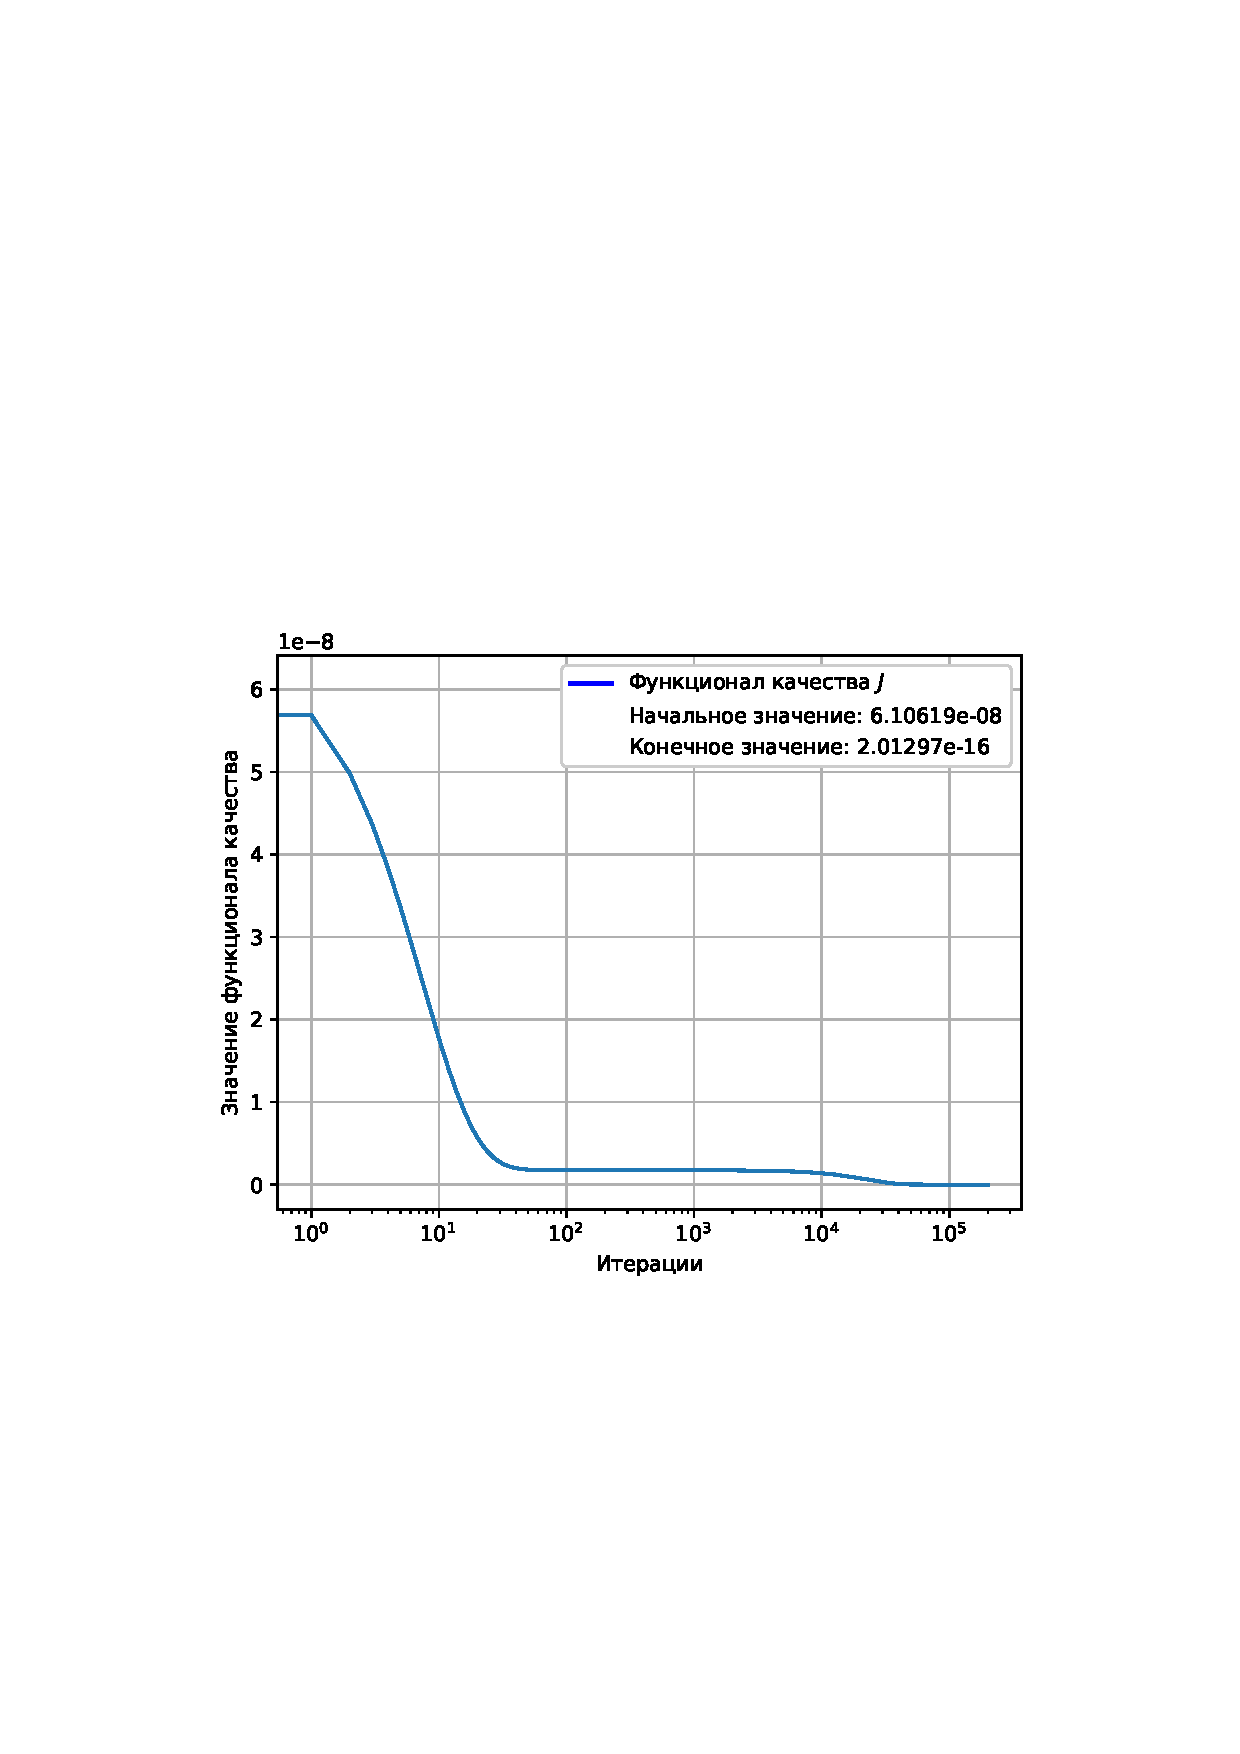
\includegraphics[width=0.8\textwidth]{cost_functional_dynamics.png}
    \caption{Dynamics of functional changes $J(\theta,u)$}
\end{figure}
\end{frame}

\begin{frame}
    \frametitle{Solution of the control problem in a semicircle}


    In this case, the considered region will be a semicircle, with a radius $1$. Function $\theta_0$ Will be chosen as the solution of the boundary problem \eqref{initial}--\eqref{initial_boundary} with $u = 0.5$
    Further on the part of the boundary lying on the abscissa axis, we change the control to $u = 0.1$.

    The region will be represented in the form:
    \begin{figure}[H]
        \centering
        \includegraphics[width=0.6\textwidth]{mesh_2.eps}
        \caption{Triangulation of the $\Omega$ domain}
    \end{figure}

\end{frame}

\begin{frame}
    \begin{figure}
        \begin{subfigure}[b]{0.5\textwidth}
        \includegraphics[width=\textwidth]{2_control.png}
        \caption{Control $\textcolor{red}{\blacksquare}$ -- $u$, $\textcolor{blue}\blacksquare$ --$u_{10000}$}
        \end{subfigure}%
        ~ %add desired spacing between images, e. g. ~, \quad, \qquad, \hfill etc.
          %(or a blank line to force the subfigure onto a new line)
        \begin{subfigure}[b]{0.5\textwidth}
        \includegraphics[width=\textwidth]{2_cost_functional_dynamics.png}
        \caption{Changes of the functional  $J(\theta)$}
        \end{subfigure}
        \caption{The result of the algorithm for finding the control function}
    \end{figure}

\end{frame}
\begin{frame}
        \begin{figure}[H]
            \includegraphics[width=0.9\textwidth]{2_theta0_and_start_and_final.png}
            \caption{Functions $\textcolor{red}{\blacksquare}$--$\theta_0$,  $\textcolor{blue}{\blacksquare}$--$\theta_1$, $\textcolor{yellow}{\blacksquare}$--$\theta_{100}$,  $\textcolor{green}{\blacksquare}$--$\theta_\text{final}$ }
            ~ %add desired spacing
        \end{figure}
\end{frame}

\begin{frame}
    \center{Thank you for your attention}
\end{frame}

\end{document}
